\documentclass[11pt,a4paper]{article}
\usepackage[T1]{fontenc}
\usepackage[utf8]{inputenc}
\usepackage{lmodern,microtype}
\usepackage[margin=25mm]{geometry}
\usepackage{amsmath,amssymb,amsthm}
\usepackage{booktabs,enumitem,graphicx}
\usepackage[round,authoryear]{natbib}
\usepackage{xcolor}
\usepackage[colorlinks=true,allcolors=blue!45!black]{hyperref}

\newtheorem{theorem}{Theorem}
\newtheorem{proposition}[theorem]{Proposition}
\newtheorem{lemma}[theorem]{Lemma}
\newtheorem{corollary}[theorem]{Corollary}
\newtheorem{conjecture}[theorem]{Conjecture}
\theoremstyle{remark}
\newtheorem{remark}[theorem]{Remark}

\newcommand{\one}{\mathbf 1}
\newcommand{\E}{\mathbb E}

\title{How much can a fractional audit overstate coalition savings?\\
Exact bounds for pooled newsvendor costs under a standalone-cost floor}
\author{Guido Morgante}
\date{Draft, 6 November 2026}

\begin{document}
\maketitle

\begin{abstract}
Producers that pool their imbalance risk, such as wind farms bidding jointly,
share the expected cost of the pooled offer and must check that no group of
them would do better on its own. Checking every coalition is hard, so the check
is often relaxed to fractional memberships. We ask how far that relaxation can
overstate the largest saving available to an actual coalition when every
producer is known to pay at least a fraction $r$ of its standalone cost and $k$
producers are excluded from the search. For equal shares we give the exact
worst case for every number of producers, every depth $k$ and every $r$: it
equals the elementary ceiling $(1-r)(n-k)/n$ on a union of explicit intervals
and is strictly smaller elsewhere, with closed forms in all regimes. For
arbitrary shares we give the exact worst case at the deepest nonterminal level
and four families of explicit worst-case laws at every depth, whose best value
matched a certified upper bound in all 1068 random instances computed. Every
bound is attained by a finite demand law. The constructions rest on the fact
that costs of symmetric demand laws are zonotope support functions; the upper
bounds rest on triangle-inequality certificates.
\end{abstract}

\section{Introduction}

Renewable producers that offer their output jointly pay imbalance penalties on
the pooled position rather than on their own. Pooling lowers the expected
penalty, and the saving must be shared. A cost split is acceptable only if no
group of producers would pay less by leaving and offering on its own: the split
must lie in the core of the pooling game \citep{baeyens2013wind,
chakraborty2018causation}. For newsvendor-type games the core is nonempty
\citep{hartman2000cores, muller2002newsvendor, montrucchio2012review}, but
deciding whether a given split lies in it is NP-hard \citep{chenzhang2009inventorygames}.

A natural tractable check replaces actual coalitions by fractional ones: a
producer may join with a fraction of its output, and the largest saving over
fractional memberships is a convex program. The fixed-allocation version of
this relaxation appears in \citet[Section~5]{burer2005centralized}; fractional
and partially continuous memberships have a long history in cooperative game
theory \citep{aubin1981fuzzy, samet1984dualcore, denault2001coherent,
bonnans2008leastcore}, and integrality gaps of relaxations are closely tied to
approximate cores in combinatorial games \citep{deng1999algorithmic,
goemans2004facility, caprara2010costsharing}. The relaxation can only
overstate the saving. The question of this paper is by how much.

Without further information the answer is discouraging: the overstatement can
be as large as the charges of the producers kept in the search
(Proposition~\ref{prop:ceilings}). But an auditor usually knows more. We assume
that every producer pays at least a fraction $r$ of its standalone cost, and
ask for the exact worst case as a function of $r$, of the shares and of the
number $k$ of producers excluded from the search.

\paragraph{Results.} For equal shares the answer is complete
(Theorems~\ref{thm:equal} and~\ref{thm:windows}, Figure~\ref{fig:curves}). The
elementary ceiling $(1-r)(n-k)/n$ is exact on a union of explicit intervals of
$r$; above $(m-1)/(m+1)$, with $m=n-k$, the worst case is
$(m-1)(1-r^2)/(2nr)$; and in the remaining ``windows'' it is the larger of two
explicit families, with a quadratic in $r$ deciding which. For arbitrary shares
the worst case at depth $n-2$ has three regimes per pair of producers
(Theorem~\ref{thm:lastdepth}). At every depth, four explicit families give
lower bounds (Theorem~\ref{thm:families}) whose maximum matched a certified
upper bound in every one of 1068 random instances, which we state as a
conjectured closed form (Conjecture~\ref{conj:closed}). With generic shares the
elementary ceiling turned out to be exact whenever $r\le 0.4$ in our samples,
and never when $r\ge 0.7$.

\paragraph{Method.} Every lower bound is attained by an explicit finite,
centrally symmetric demand law. Such laws have costs $c(x)=\sum_k p_k|x_k^\top
x|$, support functions of zonotopes, a classical identity
\citep{koshevoy1997zonoid, molchanov2012zonoid}; the constructions are lists of
generators. Every upper bound is a nonnegative combination of
triangle-inequality certificates. Requiring positive definite covariance and
strict stability of every coalition does not change any of the suprema
(Proposition~\ref{prop:mixtures}).

\begin{figure}[t]
\centering
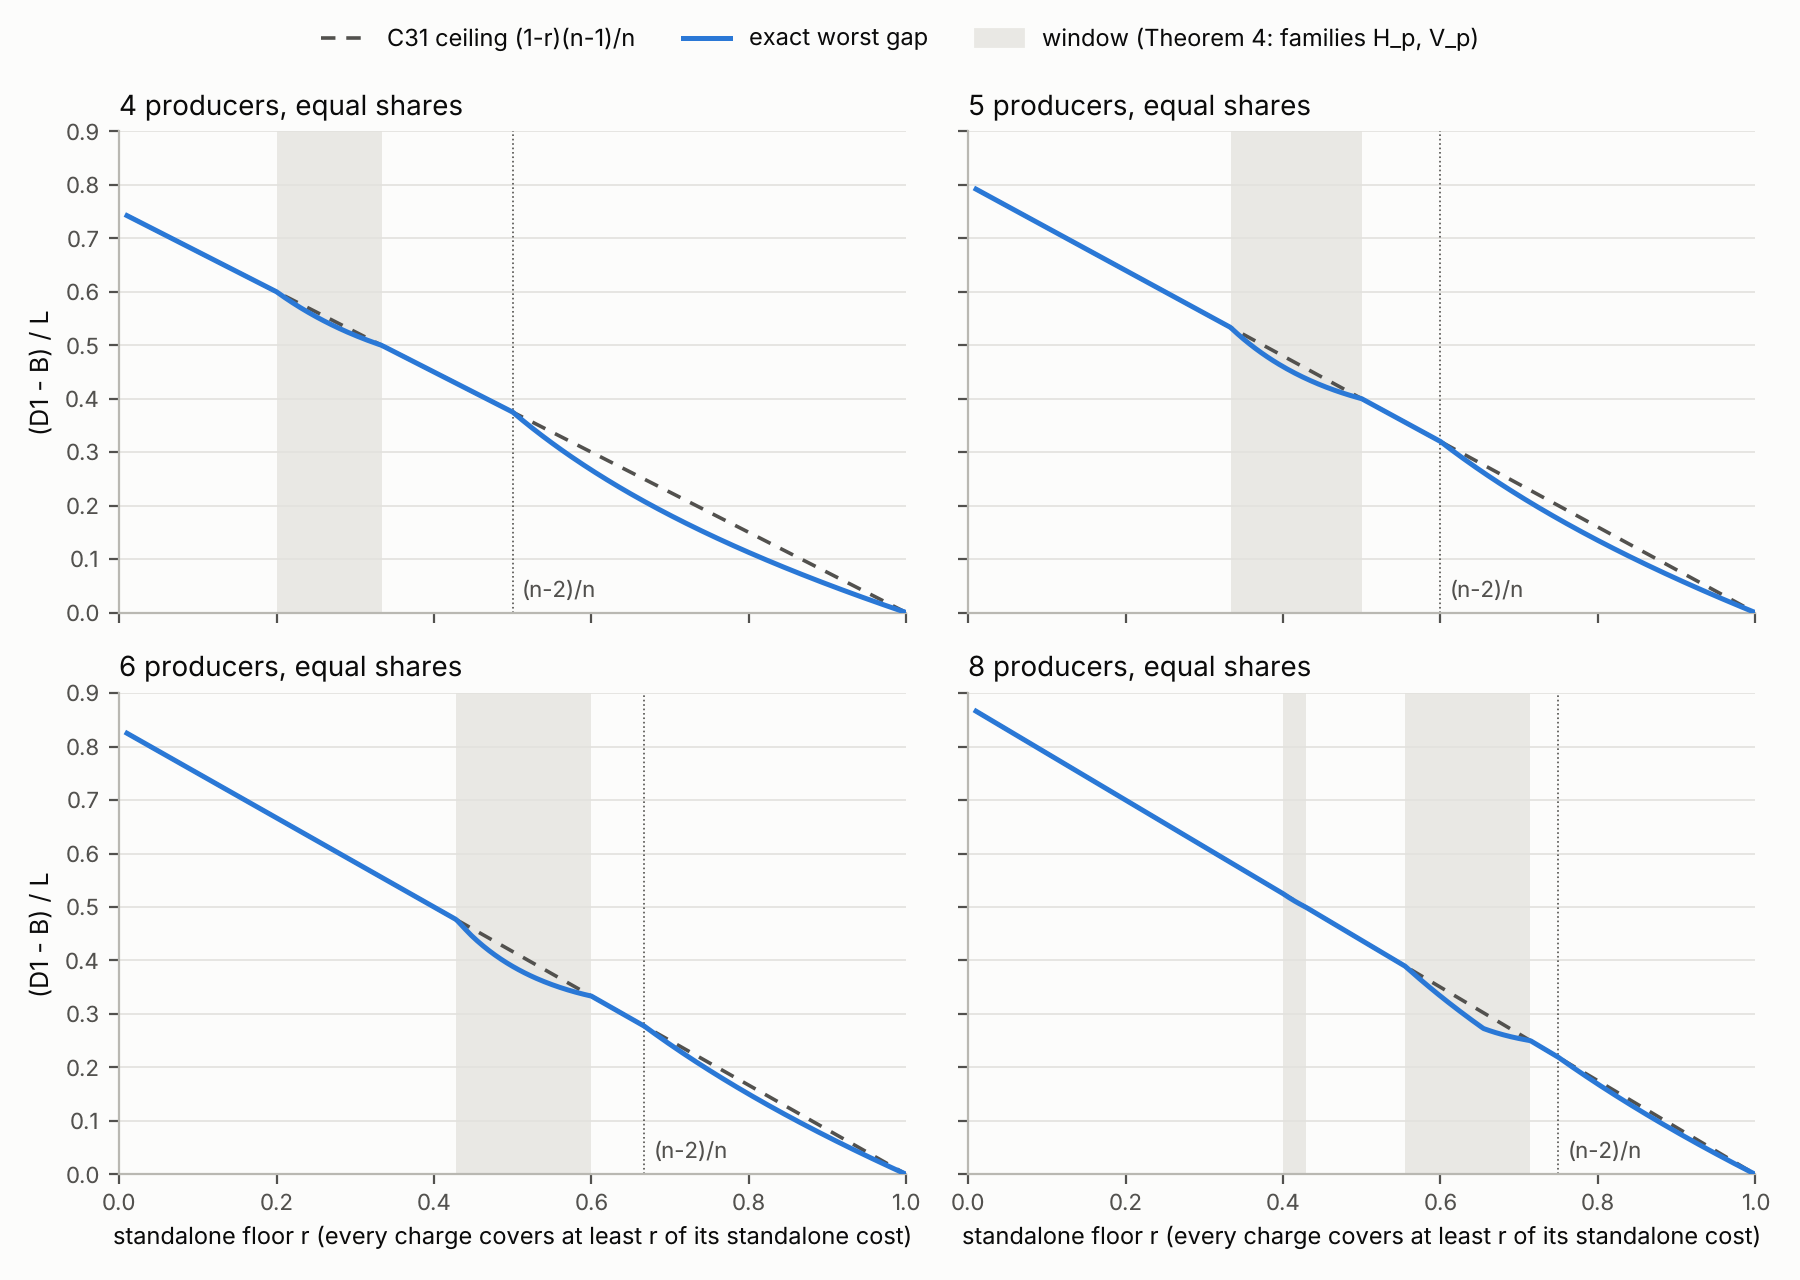
\includegraphics[width=\linewidth]{exact_envelopes.png}
\caption{Exact worst-case overstatement $(D_1-B)/L$ at depth one for equal
shares, against the standalone floor $r$, with the elementary ceiling
$(1-r)(n-1)/n$ (dashed). Shaded bands are the windows of
Theorem~\ref{thm:windows}; the dotted line marks $(n-2)/n$.}
\label{fig:curves}
\end{figure}

\section{Model}

Let $N=\{1,\dots,n\}$, $n\ge3$, and let $Y=(Y_1,\dots,Y_n)$ be bounded,
nonnegative outputs with arbitrary dependence. Imbalance is priced by the
symmetric absolute loss $\ell(q,t)=|t-q|$. For a membership vector
$z\in\mathbb R_+^n$ the \emph{physical fractional cost} is
\[
c(z)=\min_{q\in\mathbb R}\E|z^\top Y-q| .
\]
It is nonnegative, convex and positively homogeneous; with signed arguments it
is a seminorm. A frozen grand offer $q_0$ has expected cost
$L=\E|\one^\top Y-q_0|\ge c(\one)$, and producer $j$ is charged $a_j=Lw_j$ for
positive shares $w$ summing to one. We normalize $L=1$ throughout, so $a=w$.
The excess of a membership is $f(z)=a^\top z-c(z)$, the largest positive
saving of an actual proper coalition is
$B=\max\{0,\max_{\emptyset\ne S\subsetneq N}f(\one_S)\}$, and at depth $k$
the audit computes
\[
D_k=\max\Bigl\{0,\ \max_{|N\setminus S|<k}f(\one_S),\
\max_{|J|=k}\ \max_{z\in[0,1]^n,\ z_J=0}f(z)\Bigr\},
\]
so that $D_k\ge B$ and $D_{n-1}=B$. The \emph{standalone ratio} is
$\rho=\min(\{1\}\cup\{a_j/c(e_j):c(e_j)>0\})$; the floor $\rho\ge r$ means
$c(e_j)\le a_j/r$ for every $j$. We study
\[
\Gamma_k(w,r)=\sup\{(D_k-B)/L\ :\ \rho\ge r\},
\]
the supremum over bounded demand laws and frozen offers. Write $s_k(w)$ for
the sum of the $n-k$ largest shares.

\begin{proposition}[Elementary ceilings]\label{prop:ceilings}
$\Gamma_k(w,0)=s_k(w)$ for $1\le k\le n-2$, and $\Gamma_k(w,r)\le(1-r)s_k(w)$.
\end{proposition}

\begin{proof}
On a face with free set $F$, $f(z)\le a^\top z\le a(F)\le s_k(w)$ because
$c\ge0$; this bound is attained in the limit by two-state laws. For the second
statement put $x=\sum_{j\in F}a_j(1-z_j)$. Nonnegativity gives
$f(z)-B\le a(F)-B-x$; subadditivity and the caps give
$c(\one_F)\le c(z)+x/r$, hence $f(z)-B\le(1/r-1)x$. The weighted average of
the two bounds with weights $1-r$ and $r$ is $(1-r)(a(F)-B)$.
\end{proof}

The question is how much of the gap between $(1-r)s_k(w)$ and the truth
remains, and where.

\section{Two tools}

\begin{lemma}[Laws from generators]\label{lem:generators}
Let $g_1,\dots,g_m\in\mathbb R^n$. The law that picks $k$ uniformly and a sign
$\pm$ uniformly and sets $Y=\mu\pm m g_k$ has $c(x)=\sum_k|g_k^\top x|$ for
every $x$. After an affine change of units it takes values in $[0,1]^n$, and
its centre is an optimal grand offer with $L=c(\one)$.
\end{lemma}

\begin{proof}
$x^\top Y$ is symmetric about $x^\top\mu$, which is therefore an optimal offer,
and $\E|x^\top(Y-\mu)|=\sum_k|g_k^\top x|$. Scaling all outputs, offers and
costs by a common factor changes no ratio.
\end{proof}

Hence a value $V$ is attained at depth $k$ as soon as some generators satisfy
the caps $c(e_j)\le a_j/r$, stability $c(\one_S)\ge a(S)$ for every proper $S$
(so $B=0$), $c(\one)=1$, and $a^\top z-c(z)=V$ at some $z\in[0,1]^n$ with $k$
zero coordinates. All constructions below are of this form.

\begin{lemma}[Triangle certificates]\label{lem:certificates}
Let $z$ lie on a face with free set $F$, let $S\subseteq F$ and $0\le\nu\le1$.
Then
\[
f(z)-B\le a^\top z-\nu\,a(S)+\sum_{i\in S}\frac{a_i}{r}|z_i-\nu|
+\sum_{i\in F\setminus S}\frac{a_i}{r}z_i .
\]
\end{lemma}

\begin{proof}
$\nu\one_S=z-(z-\nu\one_S)$, so the triangle inequality and the caps give
$\nu c(\one_S)\le c(z)+\sum_{i\in F}(a_i/r)|z_i-\nu\one_S(i)|$, while
$c(\one_S)\ge a(S)-B$. Since $\nu\le1$, the term $\nu B-B$ is nonpositive.
\end{proof}

By positive homogeneity a maximizing membership with positive excess can be
scaled until its largest coordinate is one. With that coordinate and the order
of the others fixed, every certificate with $\nu$ equal to a coordinate is
linear in $z$, so the best bound from all of them is a linear program. It is
valid for every demand law.

\section{Equal shares}

Let $a_j=1/n$, write $M=a/r$ for the common cap, $m=n-k$ for the number of
free producers, and for $p=1,\dots,m-1$ put $q=m-p$ and
\[
I_p=\Bigl[\max\Bigl(0,\tfrac{q-p}{q+p}\Bigr),\ \tfrac{q}{q+2p}\Bigr].
\]

\begin{theorem}\label{thm:equal}
For equal shares, $1\le k\le n-2$ and $0<r\le1$,
\[
\Gamma_k=\frac{(1-r)m}{n}\quad\text{if } r\in I_1\cup\dots\cup I_{m-1},
\qquad
\Gamma_k=\frac{(m-1)(1-r^2)}{2nr}\quad\text{if } r\ge\frac{m-1}{m+1}.
\]
\end{theorem}

\begin{proof}
The first value is the ceiling of Proposition~\ref{prop:ceilings}. For the
second, combine for each fractional coordinate the certificates of
Lemma~\ref{lem:certificates} with $S$ containing or omitting it ($\nu=1$):
with the largest coordinate at one, $f(z)-B\le\sum_j h(z_j)$ where
$h(t)=\min\{(1-t)(M-a),t(M+a)\}$, and also $f(z)-B\le a^\top z$. The minimum is
concave and symmetric in the $m-1$ other coordinates, so a common value is
optimal, and a one-variable computation gives the stated value for
$r\ge(m-1)/(m+1)$.

\emph{Construction on $I_p$.} Take $p$ unit producers $I$, $q$ fractional
producers $J$, the excluded set $K$, $t=(1-r)-pr/q$, generators $a e_l$
($l\in K$) and $(Mt/p)\one_I-Me_j$ ($j\in J$), and $z=\one_I+t\one_J$. Every
generator vanishes at $z$, so $c(z)=0$ and $a^\top z=(1-r)m/n$. The unit caps
read $qt\le p$, i.e.\ $r\ge(q-p)/(q+p)$; $c(\one)=ka+qM(1-t)=1$. For a
coalition with $s$ unit, $\tau$ fractional and $\kappa$ excluded members,
$c(\one_S)-a|S|=\tau(M-a)+(q-2\tau)Mts/p-as$, bilinear in $(s,\tau)$, with
corner values $0$, $q(M-a)$, $qMt-ap\ge0$ (i.e.\ $r\le q/(q+2p)$) and $0$.

\emph{Construction for $r\ge(m-1)/(m+1)$.} Take one unit producer $u$, the
others $J$, $\delta=(M-a)/2$, $\beta=a-(m-1)\delta\ge0$, generators $\beta e_u$,
$ae_l$ ($l\in K$), $\delta e_u-Me_j$ ($j\in J$), and
$z=e_u+\frac{1-r}2\one_J$. Then $c(z)=\beta$, $c(e_u)=a$, $c(e_j)=M$,
$c(\one)=1$, and $c(\one_S)=a|S|$ when $u\in S$ and $c(\one_S)\ge a|S|$
otherwise. The excess at $z$ is the stated value.
\end{proof}

The intervals $I_p$ leave gaps when $p^2+p<m$: the \emph{window} between
$I_{p+1}$ and $I_p$ is $(r_L,r_R)$ with $r_L=(m-p-1)/(m+p+1)$ and
$r_R=(m-2p)/m$. At depth one these are $(1/5,1/3)$ for $n=4$, $(1/3,1/2)$ for
$n=5$, $(3/7,3/5)$ for $n=6$; their total length is between $0.13$ and $0.20$
for $4\le n\le30$ and decays only like $n^{-1/2}$.

Inside a window two further families compete. The family $H_p$ keeps $p$ unit
producers and puts the others at $(1-r)/2$, with positive cost at the witness;
it is valid for $r\ge(m-p)/(m+p)$ and has value
\[
H_p(r)=\frac{(m-p)(1-r^2)}{2nr}.
\]
The family $V_p$ moves one producer from unit to fractional: with
$q'=m-p-1$,
\[
t_1=\frac{(p+1)(1-r)}{2(p+1)-m(1-r)},\qquad
t_2=\frac{(p+1)r-1+t_1}{q'},\qquad
V_p(r)=\frac1n\bigl(p-1+(p+1)r+2t_1\bigr).
\]

\begin{theorem}\label{thm:windows}
Let $p^2+p<m$, $r_L\le r\le r_R$ and $Q(r)=mr^2+2(p-1)r+2+2p-m$. Then
$\Gamma_k=V_p(r)$ if $Q(r)\ge0$ and $\Gamma_k=H_{p+1}(r)$ if $Q(r)\le0$.
\end{theorem}

\begin{proof}
\emph{Laws.} For $H_{p+1}$ write $p'=p+1$ for the number of unit producers
and $q=m-p'$, and use the generators $\beta e_i$ on the units with
$\beta=((p'+q)a-qM(1+r)/2)/p'$, $ae_l$ on $K$, and $(\delta/p')\one_I-Me_j$ on
the fractional producers, where $\delta=M(1-r)/2$; the witness is
$\one_I+\frac{1-r}2\one_J$, and the stability slack is again bilinear with
corners $0$, $q(M-a)$, $0$, $0$. It is valid because
$r\ge r_L=(m-p')/(m+p')$ makes $\beta\ge0$. For $V_p$ take one
producer $*$ in transition and
\[
\gamma=\frac{M(p+1)(1-r)}{2p},\qquad
\alpha=\frac{M((p-1)+(p+1)r)}{2q'},
\]
\[
\beta=\frac{M(m(1-r)-2p)}{2q'},\qquad
\delta=-\frac{M(2(p+1)-m(1-r))}{2},
\]
with generators $(\alpha/p)\one_I+\beta e_*-Me_j$ for the other fractional
producers, $\gamma\one_I+\delta e_*$, and $ae_l$ on $K$, at
$z=\one_I+t_1e_*+t_2\one_{J'}$. All generators vanish at $z$, every free
producer sits exactly at its cap, $c(\one)=1$, and for each of the two cases
$*\in S$ and $*\notin S$ the stability slack is bilinear in the counts, with
corner values $0$, $q'(M-a)$, $p(M-a)$, $a((m-p)/r-(m+p))$ and $M-a$,
$a(p/r+p)$, $0$, $0$, all nonnegative on the window. The witness is
admissible: $t_1\le1$ is $r\ge r_L$, and $t_2\ge0$ reduces to a quadratic
inequality in $1-r$ that holds on the whole window.

\emph{Upper bounds.} With $Z_I$ the sum of the $p$ largest coordinates,
$u=z_{p+1}$ and $Y$ the sum of the rest, four certificates suffice:
nonnegative cost $F_0$; the $p+1$ largest coordinates with $\nu=1$ ($F_A$);
the whole face with $\nu=u$ ($F_B$) and with $\nu=1$ ($F_{B'}$). If
$Q(r)\ge0$, the weights $\lambda_B=1$,
$\lambda_A=(M(m-2p)-ma)/(2M)$,
$\lambda_0=(M^2(2+2p-m)+2aM(p-1)+ma^2)/(2aM)$ and the multiplier
$M(2+2p-m)+am$ on $p-Z_I\ge0$ cancel every variable; they are nonnegative
because $r\le r_R$, $Q(r)\ge0$ and $r\ge r_L$, and the resulting constant is
$V_p(r)$. If $Q(r)\le0$, the weights $\lambda_A=(M-a)/(2M)$ and a split of the
remaining $(M+a)/(2M)$ between $F_B$ and $F_{B'}$, with multipliers on
$p-Z_I\ge0$ and $1-u\ge0$, cancel every variable, and feasibility of
nonnegative weights rearranges exactly to $Q(r)\le0$; the constant is
$H_{p+1}(r)$.
\end{proof}

\begin{corollary}\label{cor:complete}
For equal shares, $\Gamma_k(w,r)$ is known in closed form for every $n$, $k$ and
$r$, and is attained by a finite symmetric law with at most $n$ generators. For
four producers at depth one,
\[
\Gamma_1=\tfrac34(1-r)\ (r\le\tfrac15),\quad
\frac{2-r+3r^2}{2(1+3r)}\ (\tfrac15\le r\le\tfrac13),\quad
\tfrac34(1-r)\ (\tfrac13\le r\le\tfrac12),\quad
\frac{1-r^2}{4r}\ (r\ge\tfrac12).
\]
\end{corollary}

At $r=1/4$, for instance, four producers who each pay at least a quarter of
their standalone cost can still face an audit that reports a saving of
$31/56\approx55\%$ of the expected pooled cost while no actual coalition
gains anything.

\section{Arbitrary shares}

\begin{theorem}\label{thm:lastdepth}
For positive shares and $0<r\le1$, $\Gamma_{n-2}(w,r)=\max_{i\ne j}\Phi_{ij}(r)$,
where, with $x=a_i/a_j$,
\[
\Phi_{ij}(r)=
\begin{cases}
a_j(1-r^2)/(2r), & x\ge(1-r)/(2r),\\
(1-r)(a_i+a_j), & (1-r)/(1+r)\le x\le(1-r)/(2r),\\
a_i(1+r)(a_i+a_j)/(ra_j+(1+r)a_i), & x\le(1-r)/(1+r).
\end{cases}
\]
\end{theorem}

\begin{proof}
At depth $n-2$ a face has two free producers; scale the witness to
$z=e_i+te_j$. Lemma~\ref{lem:certificates} with nonnegative cost, the singleton
$\{i\}$, the pair $\{i,j\}$ and, through the triangle inequality
$tc(e_j)\le c(z)+c(e_i)$, the cap of $i$, bounds the excess by the lower
envelope of $a_i+ta_j$, $ta_j(1+1/r)$, $(1-t)a_j(1/r-1)$ and
$(1-t)a_i(1+1/r)$, whose maximum over $t$ is $\Phi_{ij}$. The three regimes
are attained by the families C31, H and G of Theorem~\ref{thm:families} with
$|I|=|J|=1$.
\end{proof}

Fix an excluded set $K$, a split of the free producers into units $I$ and
fractional producers $J$, and write $a(I)$, $A_J$ for their share totals.

\begin{theorem}\label{thm:families}
For positive shares and any depth $k$, $\Gamma_k(w,r)$ is at least the largest
of the following values over all $K$ and splits:
\begin{enumerate}[label=(\alph*)]
\item C31: $(1-r)(a(I)+A_J)$ if $\frac{1-r}{1+r}A_J\le a(I)\le\frac{1-r}{2r}A_J$;
\item H: $A_J(1-r^2)/(2r)$ if $a(I)\ge\frac{1-r}{2r}A_J$;
\item G: $a(I)+tA_J$ with $t=a(I)/(rA_J+(1+r)a(I))$, if
$a(I)\le\frac{1-r}{1+r}A_J$.
\end{enumerate}
\end{theorem}

\begin{proof}
In all three families the excluded producers carry generators $a_le_l$ and the
unit coefficients are proportional to the shares. (a) With
$t=(1-r)-ra(I)/A_J$, one generator per $j\in J$ with entries
$(a_j/r)ta_i/a(I)$ on the units and $-a_j/r$ at $j$; the witness
$\one_I+t\one_J$ has zero cost, the unit caps are the lower condition, and with
$\sigma$ the unit share fraction of a coalition and $a(T)$ its fractional
share, the stability slack is bilinear with corners $0$, $A_J(1/r-1)$,
$A_Jt/r-a(I)$ and $0$. (b) With $\Delta=A_J(1-r)/(2r)$, unit generators
$(1-\Delta/a(I))a_ie_i$ and fractional generators with entries
$(a_j/r)\frac{1-r}2a_i/a(I)$ on the units and $-a_j/r$ at $j$; the slack is
$a(T)(1/r-1)(1-\sigma)\ge0$. (c) With $c_j=a_ja(I)/(rtA_J)$, generators with
entries $c_jta_i/a(I)$ on the units and $-c_j$ at $j$; the unit caps are tight,
$c(\one)=1$, the witness $\one_I+t\one_J$ has zero cost, and the slack is
bilinear with corners $0$, $A_J(\lambda-1)$, $a(I)(1/r-1)$, $0$, where
$\lambda=a(I)/(rtA_J)\ge1$.
\end{proof}

A fourth family, with one producer in transition as in $V_p$, has the value
$a(I)(1+r)-a_*(1-r)+2t_1a_*$ with
$t_1=(1-r)(a(I)+a_*)/(ra(F)+a(I)+a_*-A_{J'})$; we have not yet written
general validity conditions for it and check each candidate exactly.

\begin{conjecture}\label{conj:closed}
For positive shares, every depth $k$ and $0<r\le1$, $\Gamma_k(w,r)$ equals the
largest value of the four families over all excluded sets and splits.
\end{conjecture}

The lower bound is proved, so the conjecture concerns the upper bound. For
every instance it can be tested with the certificate linear program of
Section~3. In 1000 random instances with up to six producers, random depth
and $r$, the best family was a valid law in exact arithmetic and its value
equalled the certificate bound in all 1000 cases (C31 in 482, H in 467, the
transitional family in 27, G in 24); the same held in 68 further instances.
In those 68, the elementary ceiling $(1-r)s_k(w)$ was the answer in all 39
instances with $r\le0.4$ and in none of the 15 with $r\ge0.7$.

\section{Strict stability and positive definite covariance}

\begin{proposition}\label{prop:mixtures}
For $0<r<1$ the suprema in Theorems~\ref{thm:equal}, \ref{thm:windows},
\ref{thm:lastdepth} and~\ref{thm:families} are unchanged if the law must also
have positive definite covariance and strictly negative excess for every proper
coalition.
\end{proposition}

\begin{proof}
Let $X^s$ put mass $0.9$ evenly on the atoms $\pm s(e_i-e_j)$ over all pairs
and mass $0.1$ on $\pm\zeta\one$. With $1.8s/n>1$ every proper coalition has
$c^s(\one_S)>a(S)$, and $c^s(\one)\le1$ for small $\zeta$; its covariance is
positive definite. Mix a worst-case law at the ratio
$r'=(1-\varepsilon)/\min_j(1/r-\varepsilon c^s(e_j)/a_j)$ with $X^s$, weights
$1-\varepsilon$ and $\varepsilon$. Costs of centrally symmetric laws mix
linearly, so the mixture is strictly stable, respects the caps at $r$, has
grand cost at most one and covariance at least $\varepsilon$ times that of
$X^s$, and its excess at the witness tends to the supremum as
$\varepsilon\to0$, by continuity of the closed forms in $r$.
\end{proof}

\section{Discussion}

The elementary ceiling $(1-r)s_k(w)$ is the right answer more often than one
might expect: for equal shares on most of the range of $r$, and for generic
shares whenever producers pay a small or moderate part of their standalone
cost. Where it is not, the exact curves show how much an auditor may discount a
fractional audit, and the windows show that the correction is not confined to
large $r$ when shares are symmetric. Even with a substantial standalone floor
the audit can report savings of half the pooled cost while no coalition gains.

Three questions remain open. The upper bound in Conjecture~\ref{conj:closed};
whether the relaxation over all seminorms, which the explicit laws met in every
case we computed, always coincides with the worst case over demand laws; and
asymmetric penalties, for which costs are no longer seminorms and the tools of
Section~3 need to be rebuilt.

\paragraph{Reproducibility.} Every construction, closed form and computational
claim is checked by scripts that write their outcomes to JSON before any summary
is generated; exact rational arithmetic is used for all constructions.

\bibliographystyle{plainnat}
\bibliography{references}

\end{document}
